\documentclass[bachelor, och, labwork]{shiza}
% параметр - тип обучения - одно из значений:
%    spec     - специальность
%    bachelor - бакалавриат (по умолчанию)
%    master   - магистратура
% параметр - форма обучения - одно из значений:
%    och   - очное (по умолчанию)
%    zaoch - заочное
% параметр - тип работы - одно из значений:
%    referat    - реферат
%    coursework - курсовая работа (по умолчанию)
%    diploma    - дипломная работа
%    pract      - отчет по практике
% параметр - включение шрифта
%    times    - включение шрифта Times New Roman (если установлен)
%               по умолчанию выключен
\usepackage{subfigure}
\usepackage{tikz,pgfplots}
\pgfplotsset{compat=1.5}
\usepackage{float}

%\usepackage{titlesec}
\setcounter{secnumdepth}{4}
%\titleformat{\paragraph}
%{\normalfont\normalsize}{\theparagraph}{1em}{}
%\titlespacing*{\paragraph}
%{35.5pt}{3.25ex plus 1ex minus .2ex}{1.5ex plus .2ex}

\titleformat{\paragraph}[block]
{\hspace{1.25cm}\normalfont}
{\theparagraph}{1ex}{}
\titlespacing{\paragraph}
{0cm}{2ex plus 1ex minus .2ex}{.4ex plus.2ex}

% --------------------------------------------------------------------------%


\usepackage[T2A]{fontenc}
\usepackage[utf8]{inputenc}
\usepackage{graphicx}
\graphicspath{ {./images/} }
\usepackage{tempora}

\usepackage[sort,compress]{cite}
\usepackage{amsmath}
\usepackage{amssymb}
\usepackage{amsthm}
\usepackage{fancyvrb}
\usepackage{listings}
\usepackage{listingsutf8}
\usepackage{longtable}
\usepackage{array}
\usepackage[english,russian]{babel}

\usepackage[colorlinks=false]{hyperref}
\usepackage{url}

\usepackage{underscore}
\usepackage{setspace}
\usepackage{indentfirst} 
\usepackage{mathtools}
\usepackage{amsfonts}
\usepackage{enumitem}
\usepackage{tikz}
\usepackage{minted}

\newcommand{\eqdef}{\stackrel {\rm def}{=}}
\newcommand{\specialcell}[2][c]{%
\begin{tabular}[#1]{@{}c@{}}#2\end{tabular}}

\renewcommand\theFancyVerbLine{\small\arabic{FancyVerbLine}}

\newtheorem{lem}{Лемма}

\begin{document}

% Кафедра (в родительном падеже)
\chair{теоретических основ компьютерной безопасности и криптографии}

% Тема работы
\title{Идеалы полугрупп}

% Курс
\course{3}

% Группа
\group{331}

% Факультет (в родительном падеже) (по умолчанию "факультета КНиИТ")
\department{факультета КНиИТ}

% Специальность/направление код - наименование
%\napravlenie{09.03.04 "--- Программная инженерия}
%\napravlenie{010500 "--- Математическое обеспечение и администрирование информационных систем}
%\napravlenie{230100 "--- Информатика и вычислительная техника}
%\napravlenie{231000 "--- Программная инженерия}
\napravlenie{10.05.01 "--- Компьютерная безопасность}

% Для студентки. Для работы студента следующая команда не нужна.
% \studenttitle{Студентки}

% Фамилия, имя, отчество в родительном падеже
\author{Токарева Никиты Сергеевича}

% Заведующий кафедрой
% \chtitle{} % степень, звание
% \chname{}

%Научный руководитель (для реферата преподаватель проверяющий работу)
\satitle{аспирант} %должность, степень, звание
\saname{В. Н. Кутин}

% Руководитель практики от организации (только для практики,
% для остальных типов работ не используется)
% \patitle{к.ф.-м.н.}
% \paname{С.~В.~Миронов}

% Семестр (только для практики, для остальных
% типов работ не используется)
%\term{8}

% Наименование практики (только для практики, для остальных
% типов работ не используется)
%\practtype{преддипломная}

% Продолжительность практики (количество недель) (только для практики,
% для остальных типов работ не используется)
%\duration{4}

% Даты начала и окончания практики (только для практики, для остальных
% типов работ не используется)
%\practStart{30.04.2019}
%\practFinish{27.05.2019}

% Год выполнения отчета
\date{2022}

\maketitle

% Включение нумерации рисунков, формул и таблиц по разделам
% (по умолчанию - нумерация сквозная)
% (допускается оба вида нумерации)
% \secNumbering

%-------------------------------------------------------------------------------------------

\section{Постановка задачи}

  \textbf{Цель работы:} изучение строения полугрупп с помощью отношений Грина.
  
  Порядок выполнения работы:
    \begin{enumerate}
        \item Рассмотреть понятия идеалов полугруппы. Разработать алгоритмы построения идеалов полугруппы по таблице Кэли.
        \item Рассмотреть понятия и свойства отношений Грина на полугруппах.
        \item Разработать алгоритмы вычисления отношений Грина и построения <<egg-box>>-картины конечной полугруппы.
    \end{enumerate}

\section{Теоретические сведения по рассмотренным темам с их обоснованием}

  Пусть $S$ -- произвольная полугруппа.\\
  \textbf{Определение 1.} Полугруппа – это алгебра S = (S, ·) с одной ассоциативной бинарной
    операцией $\cdot$, т.е. выполняется
      \begin{center}
        $(x \cdot y) \cdot z = x \cdot (y \cdot z)$
      \end{center}
    для любых $x,y,z \in S$.
    
    \textbf{Определение 2.} Непустое подмножество $I \subset S$ называется правым (левым) идеалом полугруппы $S$,
    если для любых $x \in I$, $y \int S$ выполняется условие: $xy \int I$ ($yx \in I$), т.е. $I \cdot S \subset I$ ($S \cdot I \subset I$).
    Если $I$ -- одновременно левый и правый идеал полугруппы $S$, то $I$ называется двусторонним идеалом (или просто идеалом) полугруппы
    $S$. Ясно, что в коммутативной полугруппе $S$ все эти определения совпадают.

    \textbf{Лемма 1.} Множество всех идеалов $Id S$  (соответственно, левых идеалов $LId S$  или правых идеалов $RId S$) любой
    полугруппы $S$ является системой замыкания. Пусть $X$ -- подмножество полугруппы $S$. Тогда наименьший правый идеал 
    полугруппы $S$, содержащий подмножество $X$, равен $(X] = XS^1 = X \cup XS$, наименьший левый идеал полугруппы $S$, содержащий
    подмножество $X$, равен $[X) = S^1X = X \cup SX$  и наименьший идеал полугруппы $S$, содержащий подмножество $X$, равен 
    $[X] = S^1XS^1 = X \cup XS \cup SX \cup SXS$.
    
    В частности, любой элемент $a \in S$ определяет наименьшие правый, левый и двусторонний идеалы: $(a] = aS^1$, $[a) = S^1a$ и
    $[a] = S^1aS^1$, которые называются главными (соответственно, правыми, левыми и двусторонними) идеалами.
    Минимальные относительно теоретико-множественного включения идеалы (левые или правые идеалы) называются минимальными идеалами
    (минимальными левыми или правыми идеалами).
    
    \textbf{Лемма 2.} Если полугруппа имеет минимальный идеал, то он является ее наименьшим идеалом и называется ядром полугруппы.

    \underline{Пример:} В полугруппе натуральных чисел с операцией сложения $\textbf{N} = (\textbf{N}, +)$ главные идеалы 
    $(n] = {n, n + 1, n + 2, \dots}$ образуют бесконечную последовательность с пустым пересечением.

    \begin{center}
      Отображения $f: a \mapsto [a]$, $f_r: a \mapsto (a]$, $f_l: a \mapsto [a)$, $a \in S$ определяют ядра $\mathfrak{J} = ker f$,
      $\mathfrak{R} = ker f_r$, $\mathfrak{L} = ker f_l$ по формулам:

      $(a, b) \in \mathfrak{J} \Longleftrightarrow [a] = [b]$,

      $(a, b) \in \mathfrak{R} \Longleftrightarrow (a] = (b]$,

      $(a, b) \in \mathfrak{L} \Longleftrightarrow [a) = [b)$.
    \end{center}

    Все эти отношения, а также отношения $\mathfrak{D}  = \mathfrak{R} \vee \mathfrak{L}$, $\mathfrak{H}  = \mathfrak{R} \cap \mathfrak{L}$
    являются эквивалентностями на множестве $S$, которые называются \textbf{отношениями Грина} полугруппы $S$. Классы этих эквивалентностей,
    порожденные элементом $a \in S$, обозначаются $J_a$, $R_a$, $L_a$, $D_a$ и $H_a$, соответственно.
  
    \textbf{Лемма 3.} Отношения Грина полугруппы $S$ удовлетворяют следующим свойствам:

    \begin{enumerate}
      \item эквивалентность $\mathfrak{R}$ регулярна слева и эквивалентность $\mathfrak{L}$ регулярна справа, т.е.
      $(a, b) \in \mathfrak{R} \Rightarrow (xa, xb) \in \mathfrak{R}$ и $(a, b) \in \mathfrak{L} \Rightarrow (ax, bx) \in \mathfrak{L}$ 
      для любых $x \in S$;
      \item эквивалентности $\mathfrak{R}$, $\mathfrak{L}$ коммутируют;
      \item $\mathfrak{D} = \mathfrak{R} \cdot \mathfrak{L} = \mathfrak{L} \cdot \mathfrak{R}$;
      \item если полугруппа $S$ конечна, то $\mathfrak{D} = \mathfrak{J}$;
      \item любой класс $\mathfrak{D}$ эквивалентности $\mathfrak{D}$ можно изобразить с помощью следующей следующей <<egg-box>>-диаграммы,
      клетки которой являются классами эквивалентности $\mathfrak{H}$, лежащими в $\mathfrak{D}$.
    \end{enumerate}


      \begin{figure}[H]
        \centering
        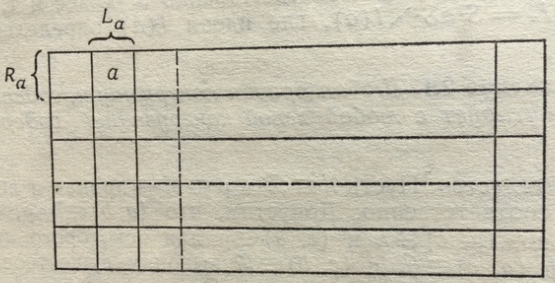
\includegraphics[width=0.8\textwidth]{photo/egg-box.png}
        \caption{<<egg-box>>-диаграмма}
      \end{figure}

\section{Результаты работы}
    \subsection{Алгоритм 1 -- Построение подполугруппы по заданному порождающему множеству}

    \textit{Вход}: Полугруппа $S$ с таблицей Кэли $A = (a_{ij})$ размерности $n \times n$ и подмножество $X \subset
    S$.

    \textit{Выход}: Подполугруппа $\langle X \rangle \subset S$.
    
    \underline{Шаг 1.} .    
    
    \underline{Шаг 2.} .
    
    \underline{Шаг 3.} .
    

        \subsection{Коды программ, реализующей рассмотренные алгоритмы}

        \inputminted[fontsize=\small]{python}{code/aua-lab5.py}

      \newpage
      
      \subsection{Результаты тестирования программ}
      
      На рисунке 1 показана работа алгоритма построения подполугруппы.

      % \begin{figure}[H]
      %   \centering
      %   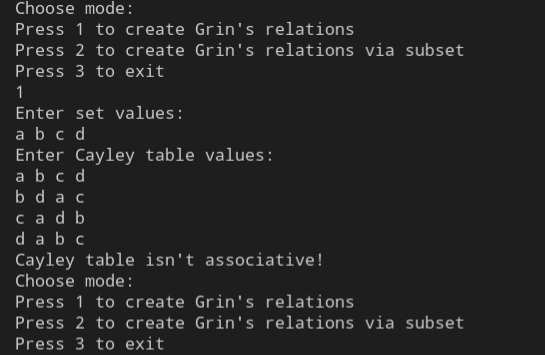
\includegraphics[width=0.8\textwidth]{photo/1.png}
      %   \caption{Тест алгоритма построения подполугруппы}
      % \end{figure}

    \subsection{Решение задач}
      \textbf{Задание 1.} Найдите подполугруппу $\langle x \rangle$, правый $(x]$, левый $[x)$ и двусторонний $[x]$ идеалы
      полугруппы $S$, порожденные элементом $x$, и определите порядок элемента x для каждого элемента полугруппы, на
      которой бинарная операция задана следующей таблицей Кэли:
        \begin{table}[H]
            \centering
            \begin{tabular}{|l|l|l|l|l|}
            \hline
            $\cdot$ & a & b & c & d \\ \hline
            a & a & b & c & d \\ \hline
            b & b & d & a & c \\ \hline
            c & a & b & d & b \\ \hline
            d & d & a & b & c \\ \hline
        \end{tabular}
        \end{table}

    \begin{enumerate}
      \item Нахождение подполугруппы:
    
      Подполугруппа строится по порождающему ее множеству. Допустим у нас есть подмножество $X \subset S$, где $X = \{ a\}$. 
      Тогда построим подполгруппу:
  
      Элемент $a$ подмножества $X$ определен в первой строчке таблицы Кэли. Поэтому мы должны пройти по элементам, находящихся в первой
      строке. Если еще такого элемента нет в подмножестве $X$, то он добавляется в данное подмножество. Т.е. пройдя по первой строке в
      данном случае получается подмножество $X = \{a, b, c, d\}$. Далее необходимо пройтись по строчкам, в котором определены новые элементы
      подмножества $X$ (т.е. $b, c, d$). Рассмотрим элемент $b$ и, пройдясь по второй строчке, видно, что новых элементов в подмножество $X$
      не добавилось. Значит, мы получили подполугруппу $\langle X \rangle = \{a, b, c, d\}$.  
    % Конечно, можно было бы обратить внимание на то, что в данном случае
    % $X = S$ и можно было бы уже и не проходить по остальным строкам таблицы Кэли, однако задачей являлось найти подполугруппу согласно алгоритму,
    % описанному в 4-й лабораторной работе.
      Аналогично строится подполугруппа для $b,c,d$ полугруппы $S$:

      Пусть $X \subset S$, где $X = {b}$. Тогда $\langle X \rangle = {a, b, c, d}$.

      Пусть $X \subset S$, где $X = {c}$. Тогда $\langle X \rangle = {a, b, c, d}$.

      Пусть $X \subset S$, где $X = {d}$. Тогда $\langle X \rangle = {a, b, c, d}$.
      
      \item Нахождение идеалов:
      
      Используя таблицу Кэли построим правые идеалы:
      
      \begin{center}

        $(a] = {a, b, c, d}$

        $(b] = {a, b, c, d}$
  
        $(c] = {a, b, d}$
  
        $(d] = {a, b, c, d}$
    
      \end{center}
    
      
      Теперь построим левые идеалы:

      \begin{center}
      
        $[a) = {a, b, d}$

        $[b) = {a, b, d}$

        $[c) = {a, b, c, d}$

        $[d) = {b, c, d}$
      \end{center}

      Также построим двусторонние идеалы:

      \begin{center}
      
        $[a] = {a, b, c, d}$

        $[b] = {a, b, c, d}$

        $[c] = {a, b, c, d}$

        $[d] = {a, b, c, d}$
        
      \end{center}


    \end{enumerate}
    
    
    \textbf{Задание 2.}
    
    Найдем отношения Грина для полугруппы $S = {a, b, c, d}$ из задания 1:

    Заполним матрицу $\mathfrak{R}$, элементы которой будут определяться следующим образом: Возьмем правый идеал $(a]$ и рассмотрим относительно
    него остальные правые идеалы. Если, например, $(a] = (b]$, то на месте пересечения элементов $a$ и $b$ в матрице $\mathfrak{R}$ будет стоять 1,
    в противном случае будет стоять 0.

    Тогда матрица будет выглядеть следующим образом:

    \begin{center}
      $\mathfrak{R} =
      \begin{pmatrix}
        1 & 1 & 0 & 1 \\
        1 & 1 & 0 & 1 \\
        0 & 0 & 1 & 0 \\
        1 & 1 & 0 & 1
      \end{pmatrix}$
    \end{center}
    
    Аналогично построим матрицу $\mathfrak{L}$ по левым идеалам:

    \begin{center}
      $\mathfrak{L} =
      \begin{pmatrix}
        1 & 1 & 0 & 1 \\
        1 & 1 & 0 & 1 \\
        0 & 0 & 1 & 0 \\
        1 & 1 & 0 & 1
      \end{pmatrix}$
    \end{center}
    
    Тогда отношение Грина будет представлено матрицей $\mathfrak{D} = \mathfrak{R} \oplus \mathfrak{L}$:

    \begin{center}
      $\mathfrak{D} =
      \begin{pmatrix}
        1 & 1 & 0 & 1 \\
        1 & 1 & 0 & 1 \\
        0 & 0 & 1 & 0 \\
        1 & 1 & 0 & 1
      \end{pmatrix}$
    \end{center}

    \textbf{Задание 3.}
    
    Найдите полугруппу $S$ по следующему ее копредставлению:
    \begin{center}

      $S = \langle x,y : xy = yx, x^3 = x, y^2 = x \rangle$
    \end{center}

    Выделим полную систему представителей классов конгруэнции $\epsilon$, которая определяется соотношениями данного
    копредставления. Для этого последовательно рассмотрим слова фиксированной длины и
    выделим те, которые не будут эквивалентны между собой относительно конгруэнции $\epsilon$.

    Рассмотрим слова длины 1: $x$, $y$ –- эти слова не эквивалентны между собой относительно конгруэнции $\epsilon$.

    Рассмотрим слова длины 2, которые получаются из слов
    длины 1 путем последовательного умножения их справа на буквы $x$ и $y$: $x^2, xy, yx = xy, y^2 = x$ -- из этих 
    слов только слова $x^2$, $xy$, не эквивалентны относительно конгруэнции $\epsilon$ другим ранее выделенным словам.

    Теперь рассмотрим слова длины 3, которые получаются из выделенных слов длины 2 путем последовательного
    умножения их справа на буквы $x$ и $y$: $x^3 = x$, $x^2y$, $xyx$,  $xy^2 = x^2$  –- из этих слов только
    слово $x^2y$ не эквивалентно относительно конгруэнции $\varepsilon$ другим ранее выделенным словам.

    Наконец рассмотрим слова длины 4, которые получаются из выделенного слова длины 3 путем последовательного
    умножения его справа на буквы $x$ и $y$: $x^3y = xy$, $x^2y^2 = x^3 = x$ -- все эти слова эквивалентны
    относительно конгруэнции $\varepsilon$ ранее выделенным словам.

        Значит, $S = \{x, y, x^2, xy, x^2y \}$ "--- полная система представителей классов конгруэнции $\varepsilon$.
        Операция умножения $\cdot$ таких слов определяется с точностью до конгруэнции $\varepsilon$ по следующей таблице
        Кэли:

     \begin{table}[H]
          \centering
          \begin{tabular}{|c|c|c|c|c|c|}
          \hline
          $\cdot $ & $x$ & $y$  & $x^2$  & $xy$ & $x^2y$ \\ \hline
          $x$      & $x^2$ & $xy$ & $x$  & $x^2y$ & $xy$ \\ \hline
          $y$      & $xy$ & $x$ & $x^2y$ & $x^2$ & $x$ \\ \hline
          $x^2$     & $x$ & $x^2y$ & $x^2$ & $xy$ & $x^2y$ \\ \hline
          $xy$    & $x^2y$ & $x^2$ & $xy$ & $x$ & $x^2$ \\ \hline
          $x^2y$   & $xy$ &  $x$  &  $x^2y$ & $x^2$ & $x^2$ \\ \hline
          \end{tabular}
        \end{table}
    \conclusion
    
    В результате лабораторной работы были рассмотрены теоретические сведения о полугруппах, подполугруппах и
    порождающих множествах. Опираясь на изложенную
    выше теорию, были разработаны алгоритмы проверки свойств операций: ассоциативность, коммутативность, идемпотентность, обратимость,
    дистрибутивность, алгоритмы построения подполугруппы по таблице Кэли, построения
    полугруппы бинарных отношений по заданному порождающему множеству, построения полугруппы по порождающему множеству и
    определяющим соотношениям. Была произведена оценка сложности каждого из  построенных алгоритмов. Была реализована программа, написанная на языке Python
    с использованием библиотеки Numpy, Math, Itertools для работы с большими массивами данных.
    
\end{document}